\section{Gamma Distribution}

\subsection{Standard Gamma Distribution}

\begin{equation}
	f(x, \alpha, \lambda) = \frac{\lambda^\alpha}{\Gamma(\alpha)} \cdot x^{(\alpha - 1)} \cdot e^{(-\lambda x)}
	\label{eq:gamma_pdf}
\end{equation}

where $\Gamma(\alpha)$ is the Gamma function. This can be written as

\begin{equation}
	f(x, \alpha, \lambda) = \exp \left[(\alpha -1)\log(x) - \lambda x + \alpha \log(\lambda) - \log(\Gamma(\alpha))\right]
	\label{eq:gamma_exp_family}
\end{equation}

with $T=(\log x, x), \eta=(\alpha, -\lambda)$ and $A(\alpha, \lambda) = \log(\Gamma(\alpha)) - \alpha  \log(\lambda)$. 

\subsubsection{Laplace Approximation of the Gamma Distribution}

To get the LPA of the Gamma function in the standard basis we need its mode and the second derivative of the log-pdf. The mode is already known to be $\hat{\theta} = \frac{\alpha -1}{\lambda}$. For the second derivative of the log-pdf we take the log-pdf and derive it twice and insert the mode for $x$:
\begin{align*}
	\text{log-pdf: } &\log\left( \frac{\lambda^\alpha}{\Gamma(\alpha)} \cdot x^{(\alpha - 1)} \cdot e^{(-\lambda x)}\right) \\
	&= \alpha \cdot \log(\lambda) - \log(\Gamma(\alpha)) + (\alpha -1)\log(x) -\lambda x\\
	\text{1st derivative: }& \frac{(\alpha-1)}{x} - \lambda \\
	\text{mode: }&  \frac{(\alpha-1)}{x} - \lambda = 0 \Leftrightarrow x=\frac{\alpha -1}{\lambda}\\
	\text{2nd derivative: }& -\frac{(\alpha-1)}{x^2}\\
	\text{insert mode: }& -\frac{(\alpha-1)}{(\frac{\alpha -1}{\lambda})^2} = -\frac{\lambda^2}{\alpha - 1} \\
	\text{invert and times -1: }&\sigma^2 = \frac{\alpha-1}{\lambda^2}
\end{align*}

The LPA of the Gamma distribution is therefore approximately distributed according to the pdf of $\mathcal{N}(\frac{\alpha - 1}{\lambda}, \frac{\lambda^2}{\alpha-1})$.

\subsection{Sqrt-Transform of the Gamma Distribution}

\subsubsection{Sqrt-Transformation}

We transform the Gamma Distribution with the Log-Transformation, i.e. $Y = \sqrt(X), g(x) = \sqrt(x), g^{-1}(x) = x^2$. The transformed pdf is

\begin{align}
f_t(x, \alpha, \lambda) &= \frac{\lambda^\alpha}{\Gamma(\alpha)} \cdot x^{2(\alpha - 1)} \cdot e^{(-\lambda x^2)} \cdot 2x \\ \nonumber
&=\frac{\lambda^\alpha}{\Gamma(\alpha)} \cdot x^{2\alpha} \cdot e^{(-\lambda x^2)}
\end{align}

which can be rewritten as

\begin{equation}
f_t(x, \alpha, \lambda) = \exp \left[2\alpha \log(x) - \lambda 2x + \alpha \log(\lambda) - \log(\Gamma(\alpha))\right]	
\label{eq:square_gamma_trans}
\end{equation}

with $T = (\log(x), x^2), \eta = (2\alpha, -\lambda)$ and $A(\alpha, \lambda) = \log(\Gamma(\alpha)) - \alpha  \log(\lambda)$. 


\subsubsection{Laplace Approximation of the sqrt-transformed Gamma Distribution}

To get the LPA of the Gamma distribution in the transformed basis we need to calculate its mode and the second derivative of the log-pdf. To get the mode we take the first derivative and set it to zero. 

\begin{align*}
\text{log-pdf: } &2\alpha \log(x) - \lambda 2x + \alpha \log(\lambda) - \log(\Gamma(\alpha)) \\
\text{1st derivative: }&  \frac{2\alpha}{x} - 2\lambda x\\
\text{mode: }& \frac{2\alpha}{x} - 2\lambda x = 0 \Leftrightarrow x = \sqrt{\frac{\alpha}{\lambda}}\\
\text{2nd derivative: }&  -\frac{2\alpha}{x^2} - 2\lambda\\
\text{insert mode: }& -\frac{2\alpha}{\frac{\alpha}{\lambda}} - 2\lambda = -4\lambda\\
\text{invert and times -1: }& \frac{1}{4\lambda}
\end{align*}

Therefore the LPA now is $\mathcal{N}\left(\sqrt{\frac{\alpha}{\lambda}}, \frac{1}{4\lambda} \right)$.

\subsubsection{The bridge for the sqrt-transformation}

We already know how to get $\mu$ and $\sigma$ from $\lambda$ and $\alpha$. To invert we calculate $\mu = \sqrt{\frac{\alpha}{\lambda}} \Leftrightarrow \alpha = \frac{\mu^2}{\lambda}$ and insert $\lambda=\frac{4}{\sigma^2}$. In summary we have

\begin{align}
\mu &= \sqrt{\frac{\alpha}{\lambda}} \\
\sigma^2 &= \frac{1}{4\lambda} \\
\lambda &= \frac{4}{\sigma^2} \\
\alpha &= \frac{(\sigma\mu)^2}{4} 
\end{align}

\begin{figure}[!htb]
	\centering
	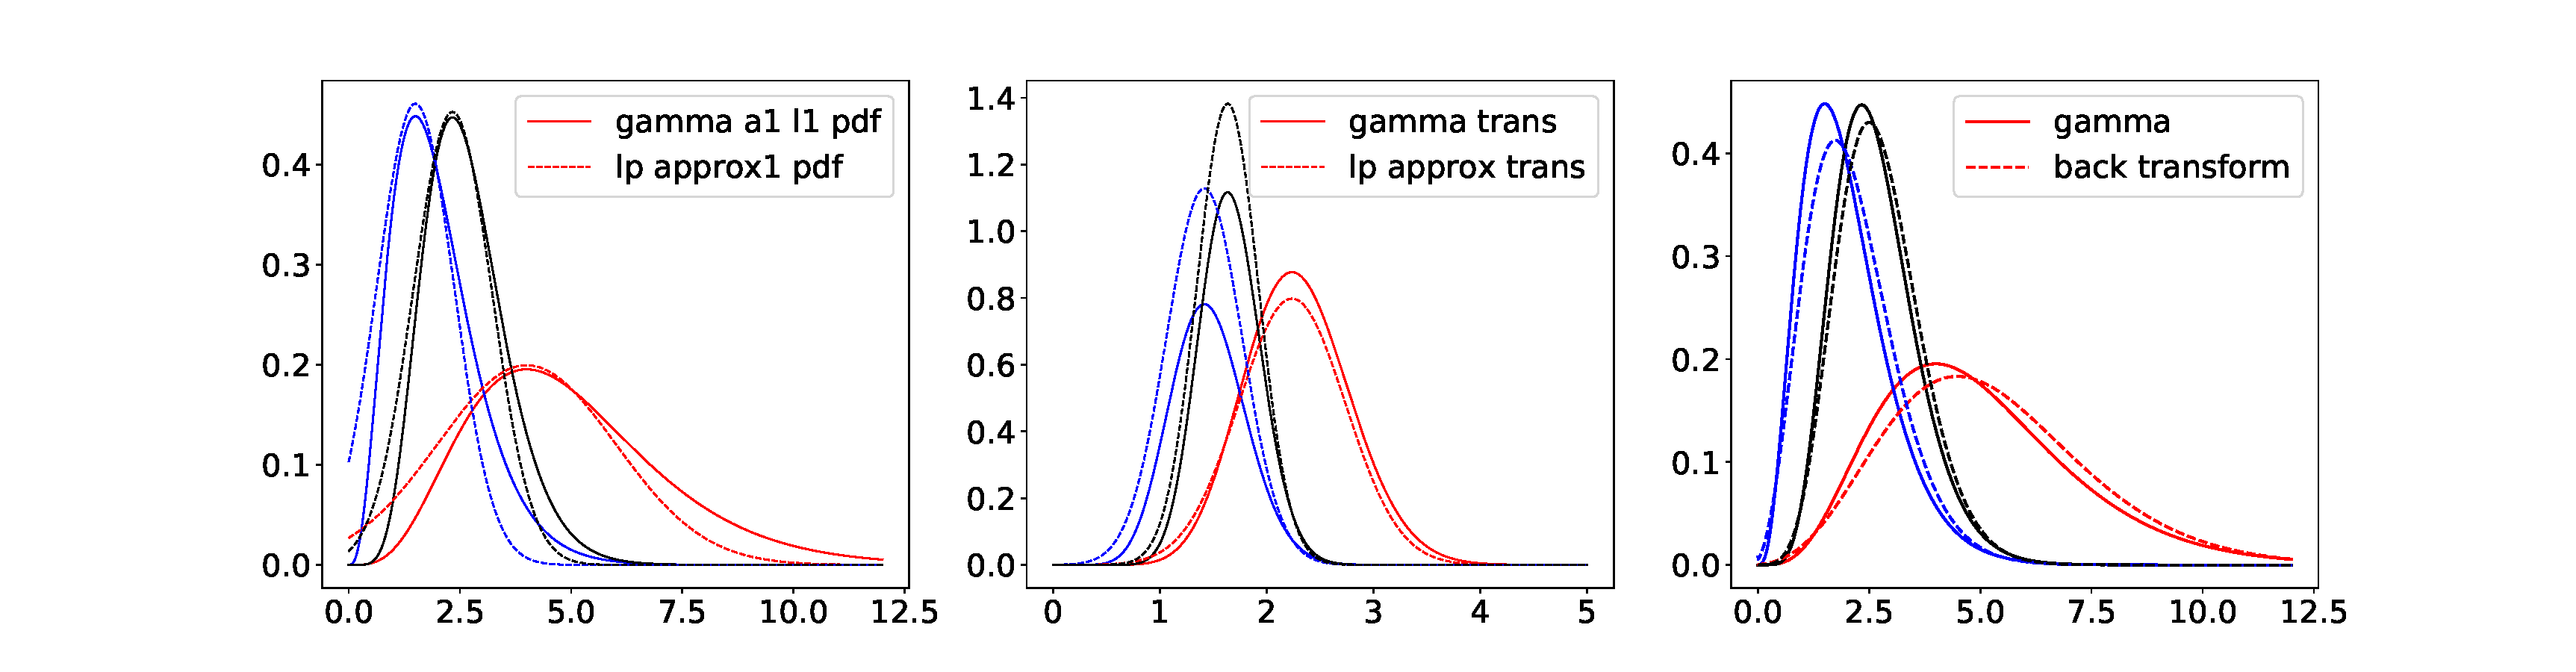
\includegraphics[width=\textwidth]{figures/gamma_playground_sqrt.pdf}
	\caption{gamma comparison square}
	\label{fig:gamma_comparison_square}
\end{figure}

\subsection{Log-Transform of the Gamma Distribution}

\subsubsection{Log-Transformation}

We transform the Gamma Distribution with the Log-Transformation, i.e. $Y = \log(X), g(x) = \log(x), g^{-1}(x) = \exp(x)$. The transformed pdf is

\begin{align}
f_t(x, \alpha, \lambda) &= \frac{\lambda^\alpha}{\Gamma(\alpha)} \cdot \exp(x)^{(\alpha - 1)} \cdot e^{(-\lambda \exp(x))} \cdot \exp(x) \\ \nonumber
&=\frac{\lambda^\alpha}{\Gamma(\alpha)} \cdot \exp(x)^{\alpha} \cdot e^{(-\lambda \exp(x))}
\end{align}

which can be rewritten as

\begin{equation}
	f_t(x, \alpha, \lambda) = \exp \left[\alpha x - \lambda \exp(x) \alpha \log(\lambda) - \log(\Gamma(\alpha))\right]	
	\label{eq:exp_gamma_trans}
\end{equation}

with $T = (x, \exp(x)), \eta = (\alpha, -\lambda)$ and $A(\alpha, \lambda) = \log(\Gamma(\alpha)) - \alpha  \log(\lambda)$. 


\subsubsection{Laplace Approximation of the log-transformed Gamma Distribution}

To get the LPA of the Gamma distribution in the transformed basis we need to calculate its mode and the second derivative of the log-pdf. To get the mode we take the first derivative and set it to zero. 

\begin{align*}
\text{log-pdf: } &\log\left(\frac{\lambda^\alpha}{\Gamma(\alpha)} \cdot \exp(x)^{\alpha} \cdot exp(-\lambda \exp(x)) \right) \\
&= \alpha \log(\lambda) - \log(\Gamma(\alpha)) + \alpha x - \lambda \exp(x)\\
\text{1st derivative: }&  \alpha - \lambda \exp(x)\\
\text{mode: }& \alpha - \lambda \exp(x) = 0 \Leftrightarrow x = \log\left(\frac{\alpha}{\lambda}\right)\\
\text{2nd derivative: }&  -\lambda \exp(x)\\
\text{insert mode: }& -\lambda \exp(\log\left(\frac{\alpha}{\lambda}\right)) = -\frac{1}{\alpha} \\
\text{invert and times -1: }&\sigma^2 = \alpha 
\end{align*}

Therefore the LPA now is $N(\log\left(\frac{\alpha}{\lambda}\right), \alpha)$.

\subsubsection{The bridge for the log-transformation}

We already know how to get $\mu$ and $\sigma$ from $\lambda$ and $\alpha$. To invert we calculate $\mu = \log(\alpha/\lambda) \Leftrightarrow \lambda= \alpha/\exp(\mu)$ and insert $\alpha=\sigma^2$. In summary we have

\begin{align}
	\mu &= \log(\alpha/\lambda) \\
	\sigma^2 &= \alpha \\
	\lambda &= \alpha/\exp(\mu) \\
	\alpha &= \sigma^2
\end{align}

\begin{figure}[!htb]
	\centering
	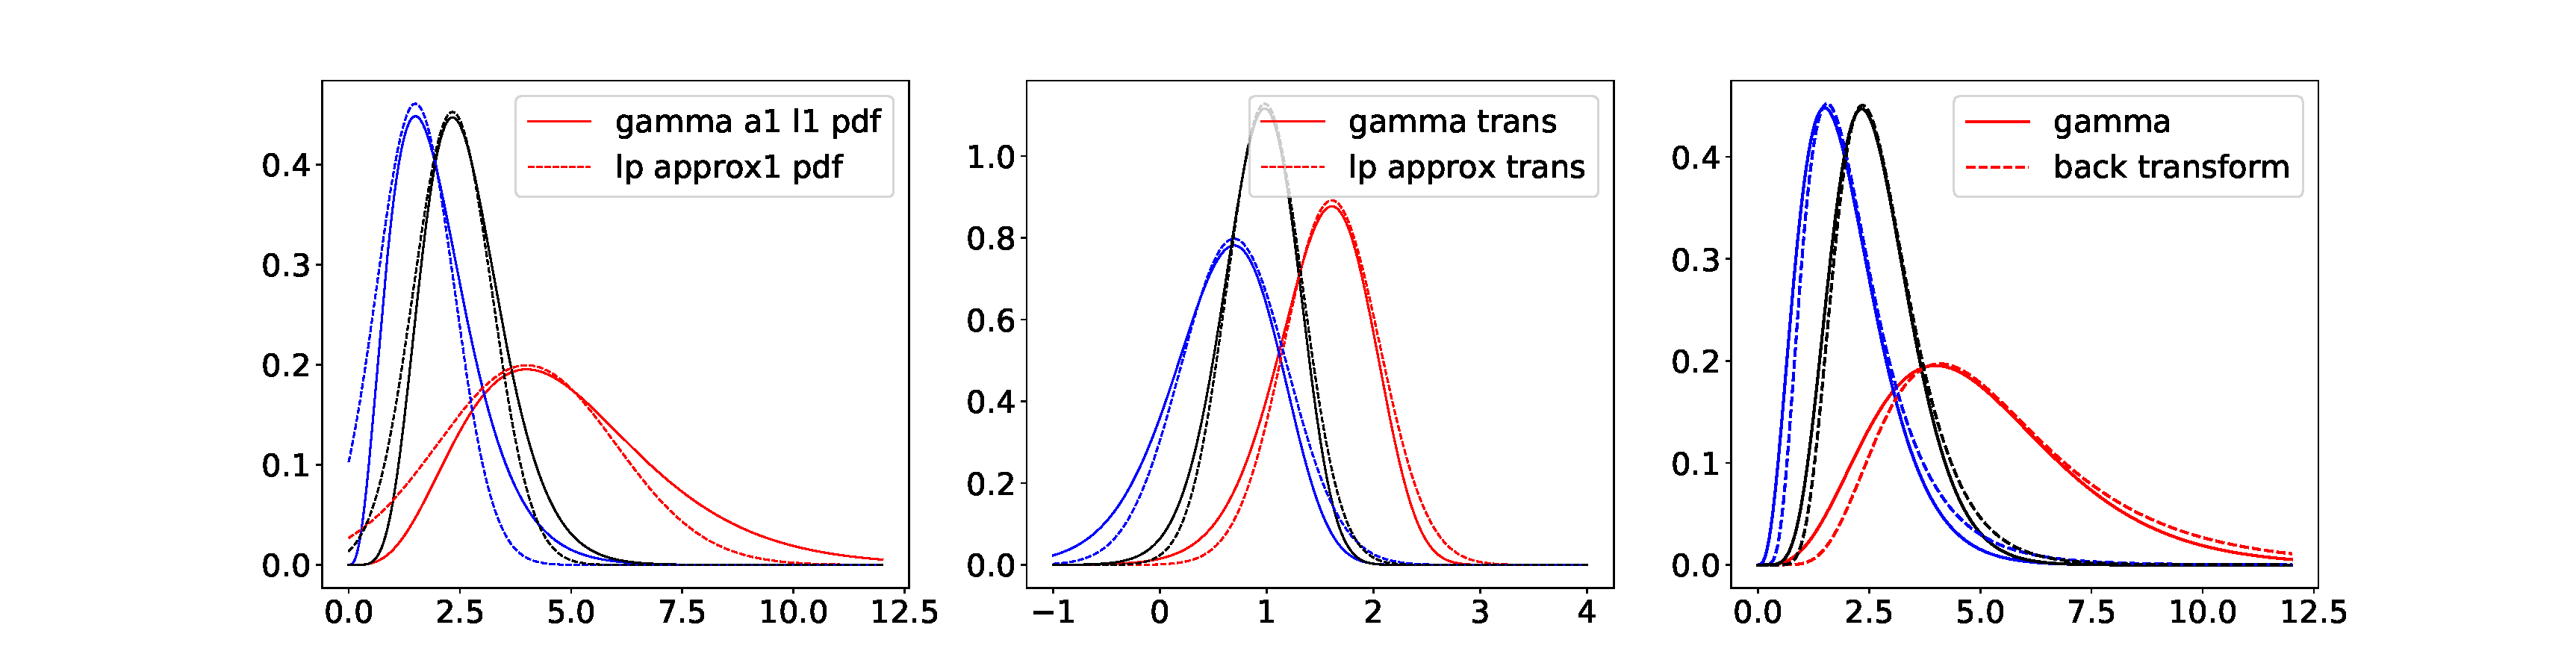
\includegraphics[width=\textwidth]{figures/gamma_playground_log.pdf}
	\caption{gamma comparison}
	\label{fig:gamma_comparison}
\end{figure}